\documentclass[12pt]{report}
\usepackage{xcolor} % for different colour comments
\usepackage{parskip} % Space between each paragraph.
%\usepackage{hardwrap} % for text length of 80 pts
\usepackage[margin=1.2in]{geometry}
\usepackage{hyperref}
\usepackage{../ltx/edcomms}
\usepackage{graphicx}
\usepackage[section]{placeins} % Prevents floats from floating across sections
\usepackage{natbib}%Bibtex
\usepackage{float}
\usepackage{tabularx}
\usepackage{ltablex} %% Multi page tables 
\usepackage{booktabs}
\usepackage{tabto}
\usepackage{tocloft} %% This package prevents table of contents from generating a page break
\usepackage{caption}
\usepackage{ifthen}
\usepackage{../ltx/edcomms}

%% Comments are enabled and disabled by 'draft' mode. I hacked in my own draft
%% mode (https://en.wikibooks.org/wiki/LaTeX/Macros) because the LaTeX draft
%% mode disables a bunch of things that I don't want it to. I just want it to
%% disable comments. Do not set any of this manually, just use the build script,
%% which builds both draft and final copies. Comments are enabled by default, so
%% if you build manually, you get a draft copy. 
\providecommand\draftmode{true}

\ifthenelse{\equal{\draftmode}{true}}{
\newcommand{\authornote}[3]{\textcolor{#1}{[#3 ---#2]}}
\newcommand{\todo}[1]{\textcolor{red}{[TODO: #1]}}
%\edcommstrue %% Dr. Kahl's comment package. Eventually we should migrate all
             %% comments to this.
}{
\edcommsfalse 
\newcommand{\authornote}[3]{}
\newcommand{\todo}[1]{}
}

% wss = Dr. Smith ; ds = Dr. Szymczak
\newcommand{\wss}[1]{\authornote{magenta}{SS}{#1}}
\newcommand{\ds}[1]{\authornote{blue}{DS}{#1}}


\usepackage{geometry}
\usepackage{changepage}
\usepackage{adjustbox}
\setlength{\parindent}{15pt} % parskip sets this to 0. 15 is default.

\newcolumntype{C}[1]{>{\centering}p{#1}} %% For use with tabularx
%%%%%%%%%%%%%%%	START OF DOCUMENT %%%%%%%%%%%%%%%%%%%%
\edcommsfalse
\begin{document}

\pagenumbering{roman} %% Roman numerals before actual document starts
\begin{titlepage}\begin{center}
\thispagestyle{empty} %% No page no. on title

\vspace*{1cm}

{\Huge\textbf{Ampersand Event-Condition-Action Rules}}

\vspace{0.5cm}
{\Large Software Requirement Specification 
	
	\edinsert{JG}{Version 0}

\vspace{1.5cm}
Yuriy Toporovskyy,\ Yash Sapra,\ Jaeden Guo}
\vfill

We acknowledge that this document uses material from the Volere Requirements
Specification Template, copyright 1995 - 2012 the Atlantic Systems Guild
Limited.

\vspace{0.8cm}
\end{center}
CS 4ZP6 \\
February 13th, 2016 \\ 
Fall 2015 / Winter 2016 
\end{titlepage}

%% Revision history

\begin{table}[ht!]\begin{center}
\caption{Revision History}  
\begin{tabular}{|l|l|l|}\hline
\textbf{Author} & \textbf{Date} & \textbf{Comment} \\\hline 
Yuriy Toporovskyy & 26 / 09 / 2015 & Initial skeleton version \\\hline
Yuriy Toporovskyy & 30 / 09 / 2015 & Project drivers, description and \\ & & 
added project diagram and project flow chart \\\hline
J Guo & 09 / 10 / 2015 & Update: Non-Functional first half 4.1-4.3, added to 
1.2.2, \\ & & completed 2.2 \\\hline
J Guo & 13 / 10 / 2015 & Update: Figures added for Non-Functional 4.1-4.7,  \\ 
& & 
Non-Functional second half 4.4-4.7 half, \\ & & added Functional 3.3 - System 
requirements  and \\ 
& & diagram figure, \& Section 5.8 \\\hline
Yash Sapra &  12/ 09 / 2015 & Non-Functional - legal requirements, \\ & & Functional - User 
Requirements, tasks, risks \\ & & and chapter 5.
\\\hline
Yuriy Toporovskyy & 13 / 10 / 2015 & Initial round of editing \\\hline
\end{tabular}
\end{center}\end{table}

\newpage

\tableofcontents
\listoffigures
\listoftables

\newpage
\pagenumbering{arabic} %% Arabic numerals in actual document

%%%%%%%%%%%%%%%%%%%%%%%%%%%%%%%%%%%%
%% Chapter 1: ???                 %%
%%%%%%%%%%%%%%%%%%%%%%%%%%%%%%%%%%%%
\setlength{\arrayrulewidth}{0.35mm}
\setlength{\tabcolsep}{16pt}
\renewcommand{\arraystretch}{2}
\begin{figure}
	\begin{adjustwidth}{-1cm}{}
	\begin{tabular}{ |m{4cm}|m{6cm}|m{4cm}|  }
		\hline
		\multicolumn{3}{|c|}{\bfseries{Project Time Table}} \\
		\hline
		\bfseries{Projected Finish Date}& \bfseries{Milestone} & 
		\bfseries{Actual Finish Date} \\
		\hline
		 09/10/2015& EFA SRS version 0 & 13/10/2015 \\
		19/10/2015 & EFA SRS version 1  & 22/10/2015 \\
		11/02/2016 & Software Demonstration & 11/02/2016 \\
        %%--- & --- & --- \\
        01/04/2016 & EFA Complete & --- \\
		\hline
	\end{tabular}
	\end{adjustwidth}
\end{figure}
\chapter{Project Drivers}\label{ch:Intro}
{\section{The Purpose of the Project}\label{sec:Purpose}}

%% 1a. The User Business or Background of the Project Effort
A large part of designing software systems is requirements engineering. One
of the greatest challenges of requirements engineering is translating from
business requirements to a functional specification. Business requirements are
informal, with the intention of being easily understood by humans; however,
functional specifications are written in formal language to unambiguously capture attributes of the 
information system. Typically, this translation
of business requirements to a formal specification is done by a requirements
engineer, which can be prone to human error.

Ampersand is a tool which aims to address this problem in a different way; by
translating business requirements written in natural language into a formal
specification by means of a ``compilation process'' (\cite{derFun}). 
Even though the business requirements and formal specification are written in
entirely different languages, the ``compiler guarantees compliance between the
two'' (\cite[2]{derFun}). 

Ampersand also provides engineers with a variety of aids which
help them to design products that fulfill all of the needs of their clients and
the end-users (Figure~\ref{fig:figure1}); including data models, service catalogs and their
specifications. Requirements engineering is perhaps most important in
safety-critical systems; to this end, Ampersand generates modeling aids and
specifications which are provably correct (\cite{derFun}). 

\begin{figure}
  \centering
    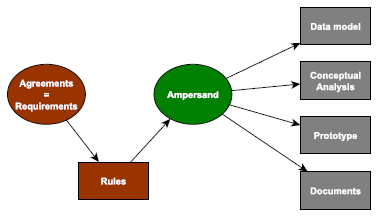
\includegraphics[width=0.7\textwidth]{../figures/ampersand_artifacts}
\caption{Ampersand produces a set of artifacts based on user's requirements.}~\label{fig:figure1}
\end{figure}

Ampersand has proven reliable in practical situations, and there have been
efforts to teach this approach to business analysts. A large portion of the
Ampersand system is already in place; the primary focus of this project is to
augment Ampersand with increased capabilities for automation.

For example, consider a system for ordering products online. Ampersand takes, as
an input, statements of business requirements like

\begin{quotation}
\noindent{\emph{Every order must have a customer and a list of products; and the total price on
the order must equal the sum of the prices of the products.}}
\end{quotation}

The requirements engineer formalizes this requirement
as a rule in Ampersand, which is a constraint on the data in the database.
These constraints are called invariants, because they are meant to remain satisfied at
all times during runtime.

 The Ampersand compiler translates each rule into Event-Condition-Action Rules (referred to as ECA rules hereafter).
An ECA-rule specifies the action to be taken by the system when an event takes place
under a given condition. In Ampersand, the purpose of an ECA-rule is to restore
invariants, i.e. to change data in the database such that the constraint becomes true
again, after having been violated. Currently, an information system generated by
Ampersand produces runtime events that signal violations of the constraints. 

It also contains the ECA rules that are generated by the Ampersand compiler --
information about ECA rules is propagated through the pipeline of Ampersand. 
However, these ECA rules are not being called in order to restore
violations automatically in the current version of Ampersand. This is due to the
fact that it is currently unclear how to incorporate the functionality of ECA
rules into the information system generated by Ampersand. 

The information system may contain a function for manipulating orders. (Ampersand can also generate
prototype software models, including functions types like these, from business
requirements - but this is not the topic of our contribution). For example,

\begin{verbatim}
addToOrder : ( o : Ref Order, t : Product )
\end{verbatim}
\noindent{where \verb|Ref x| represents the type of references to values of type
\verb|x|; \verb|Order| and \verb|Product| the types of orders and products, respectively.  }

Ampersand can generate pre- and post-conditions for this function, based on the
business requirements. This constitutes a formal specification of the
information system. For example, the above function may have the following specification:

\begin{verbatim}
{ PRE: o.totalCost = t0 } 
addToOrder(o,t) = ...
{ POST: o.totalCost = t0 + t.cost } 
\end{verbatim}

It is proven that for the subset of processes which Ampersand can support, 
there is an algorithm which will generate the necessary code to satisfy the 
post-conditions (i.e. formal specifications) of each function. However, 
Ampersand does not yet implement this algorithm. Currently, a user of Ampersand 
must manually indicate how each violation must be corrected.

In the previous example, the implementation of the
function could be as follows: 

\begin{verbatim}
{ PRE: o.totalCost = t0 } 
addToOrder(o,t) = 
  o.orders.append(t);
  o.totalCost = o.totalCost + t.cost;
{ POST: o.totalCost = t0 + t.cost } 
\end{verbatim}

The first line includes the item in the order, and the second line fixes the
violation of the post-condition which would occur without it. Currently this
second line would have to be hand-written by the programmer, but the
aforementioned algorithm can derive it from the business rules. The main
contribution of this project will be to implement the algorithm which generates
the code to fix violations.

\ds{You may want to simplify the introduction a bit to make the purpose more clear.}

\section{The Stakeholders}\label{sec:Stakeholders}
\subsection{The Client: Ampersand Designers}\label{subsec:Ampersand}
Ampersand designers are our clients and hold a stake in EFA's completion 
because it brings Ampersand one step closer to completion. The Ampersand 
designers have made provable correctness and maintainability as a part of the 
necessary conditions for EFA to be incorporated into Ampersand. The completion 
and acceptance of EFA would mean a permanent maintainable component for 
Ampersand to replace their current solution (i.e. the exec-engine) which acts 
as a temporary stand-in until a more maintainable solution can be found.


\subsection{The Customer: Ampersand Users}\label{subsec:BusReq}
\paragraph{}
EFA users are Ampersand users. EFA's contribution decreases the amount of time 
Ampersand users spend manually inserting PHP code to restore system invariants. 
This would save time for Ampersand users and make the Ampersand system more 
efficient over all.

\ds{This entire section (1.2) has been unnecessarily verbose. A simple 
explanation	of who the stakeholder is and why they hold a stake would be 
enough.}
%%%%%%%%%%%%%%%%%%%%%%%%%%%%%%%%%%%%
%% Chapter 2: Project Constraints %%
%%%%%%%%%%%%%%%%%%%%%%%%%%%%%%%%%%%%
\chapter{Project Constraints}\label{ch:Constraints}

\ds{Lack of a constraint is not a constraint.}
\edcomm{JG}{Possibly addressed?}

\section{Mandated Constraints}\label{sec:Constraints}
Due to the long-term nature of this project, external dependencies must be 
minimized. Since EFA is meant to fit within the current Ampersand system, many 
design decisions are predetermined, such as the choice of implementation 
language, what is taken as input (i.e. ECA rules) and produced as output (i.e. 
SQL queries). Additional constraints for EFA include the need for backwards 
compatibility and agreement with other modules.
%%%%%%%%%%%%%%%%%%%%%%%%%%%%%%%%%%%%%%%%%%%%%%%%%%%%%%%%%%%%%%%%%%%%%%%%%%%%%%
%%                        Solution constraints. 
%%%%%%%%%%%%%%%%%%%%%%%%%%%%%%%%%%%%%%%%%%%%%%%%%%%%%%%%%%%%%%%%%%%%%%%%%%%%%%
\subsection{Solution Constraints}\label{subsec:SolutionConstraints}
GHC 7.10  and the Cabal build system 4.22 \ref{GHC} must be used to compile all 
implemented code, and all implemented code must be in Haskell. Backwards 
compatibility is tested on older versions of Ampersand, and agreement with 
other modules are tested with system tests.

\subsection{Partner or Collaborative Applications}\label{subsec:Collaborative}
This section provides a brief description of the modules that EFA uses. More 
details are provided in the Module Guide for EFA.

\begin{adjustbox}{center}
\begin{tabular}{ |p{3.2cm}|p{11cm}|  }
    \hline
    \multicolumn{2}{|c|}{\bfseries{\large{Ampersand Core Modules}}} \\ 
    \hline\hline
    \bfseries{Module Name} & \bfseries{Description}\\
    \hline
    AbstractSyntaxTree   & Ampersand's abstract representation of input from 
    ADL.   \\
    \hline
    FSpec &   A module that represents the F-Spec structure.\\
    \hline
    Basics & An Ampersand internal module that provides basic functions for 
    data manipulation.\\
    \hline
    ParseTree    & Ampersand parse tree for ADL script; concrete representation 
    of the input, and retains all information of the input. \\
    \hline
\end{tabular}
\end{adjustbox}


\begin{adjustbox}{center}
\begin{tabular}{ |p{3.2cm}|p{11cm}|  }
    \hline
    \multicolumn{2}{|c|}{\bfseries{\large{External Haskell Modules}}} \\
    \hline\hline
    \bfseries{Module Name} & \bfseries{Description}\\
    \hline
    GHC.TypeLits   & Internal GHC module used in the implementation of 
    type-level natural numbers \cite{hackage}    \\ 
    \hline
    Data.List & A module that provides support for operations on list 
    structures.  \\
    \hline
    Data.Char &  A module that provides support for characters and operations 
    on characters.  \\
    \hline
    Data.Coerce  & Provides safe coercions between data types; allows user to 
    safely convert between values of type that have the same representation 
    with no run-time overhead \cite{hackage}.\\
    \hline
    Debug.Trace &  Interface for tracing and monitoring execution, used for 
    investigating bugs and other performance issues \cite{hackage}. \\ 
    \hline 
    GHC.TypeLits & Internal GHC module that declares the constants used in 
    type-level implementation of natural numbers \cite{hackage}.  \\ 
    \hline  
    SimpleSQL.Syntax&   The AST for SQL queries \cite{hackage}\\ 
    \hline
    Text.PrettyPrint .Leijen & A pretty printer module based 
    off of Philip Wadler's 1997 "A prettier printer", used to show SQL queries 
    in a readable manner to humans \cite{hackage}.\\ 
    \hline
    GHC.Exts & This module provides access to types, classes, and functions 
    necessary to use GHC extensions. \\ 
    \hline
    Unsafe.Coerce &  A helper module that converts a value from any type to any 
    other type.This is used in the translation of ECA rules to SQL using 
    user-defined data types. \\ 
    \hline
     System.IO.Unsafe & IO computation must be free of side effects and 
     independent of its environment to be considered safe. Any I/O computation 
     that is wrapped in unsafePerformIO performs side effects. \\
    \hline
\end{tabular}
\end{adjustbox}

\begin{adjustbox}{center}
    \begin{tabular}{ |p{3.2cm}|p{11cm}|  }
        \hline
        \multicolumn{2}{|c|}{\bfseries{\large{EFA Modules}}} \\
        \hline\hline
        \bfseries{Module Name} & \bfseries{Description}\\
        \hline
        ECA2SQL & The top-level module that takes ECA rules from FSpec and 
        converts it into SQL queries.    \\ 
        \hline
        Equality & Various utilities related to type level equality   \\ 
        \hline
        PrettyPrinterSQL & Prints SQl queries in human-readable format    \\ 
        \hline
        Singletons & Module for Singleton datatypes, the module defines 
        singleton for a kind in terms of an isomorphism between a type and a 
        type representation   \\ 
        \hline
        Trace & Provides trace messages and various utilities used by 
        ECA2SQL    \\ 
        \hline
        TSQLCombinators & Uses an overloaded operator for indexing and 
        implements SQL as a primitive data type.   \\ 
        \hline
        TypedSQL & Contains basic SQL types represented in Haskell.    \\ 
        \hline
        Utils & Provides utility functions for ECA2SQL and contains type 
        families    \\ 
        \hline
    \end{tabular}
\end{adjustbox}
\subsection{Off-the-Shelf Software}\ref{subsec:Off-the-ShelfSol}
Open source software used to implement EFA modules include the Glasgow Haskell 
Compiler with the Cabal system (\ref{GHC}). 

\subsection{Schedule Constraints}
\begin{itemize}
    \item To meet software completion deadline by April 2016
    \item To meet all necessary deadlines for Capstone project 
\end{itemize}

\subsection{Project philosophy}

Any code submitted must be well-documented, backwards-compatible and 
mathematically provable. Project code must satisfy existing tests, and 
additional tests should be written for the new algorithm being implemented. 

\ds{So the code must be well-documented and backwards-compatible?}

%%3b.
\subsection{Implementation environment}\label{subsec:ImplementationEnvironment}
\subsubsection*{Haskell}
The Ampersand code base is written almost entirely in Haskell 
(\cite{ampSource}) with the exception of user interfaces for the generated 
prototypes written in PHP and Javascript. Additional PHP code may be required 
for the prototype, however Haskell is the main programming 
language we use to build modules for Ampersand. 

\subsubsection*{The Glasgow Haskell Compiler \& Cabal build}\label{GHC}
The Glasgow Haskell Compiler 7.10 (\cite{GHC}) together with the Cabal build 
system (see \verb|ampersand.cabal| must be used to compile Ampersand 
\cite{ampSource}). Ampersand is not designed to used with other Haskell 
compilers.

\ds{This doesn't sound like a constraint}
\edcomm{JG}{Dont know what this was in reference to anymore ..}



\subsubsection*{GitHub}\label{Github}
Github hosts the most current version of the Ampersand system. Github is used 
to maintain consistency between the main Ampersand branch and this project.

\edcomm{YS}{Do we want to tell them that our code might not be integrated in 
Ampersand?
I think we should abstract this information to make our configuration look more significant.}%

\subsubsection*{Graphviz}
Graphviz is an open source graph visualization software, which can
visually represent information in the form of charts and graphs. It contains
various designs from which the user is able to select. This is used to take
descriptions of graphs in simple text and create diagrams. Ampersand generates
reports about the input system using graphs and charts, thus Graphviz is one of 
the basic components required to produce Ampersand artifacts.

\subsubsection{The Cabal System}
The Cabal system is for building and packaging Haskell libraries and programs. 
Cabal describes what a Haskell package is, how these packages interact with the 
language, and what Haskell implementations must do to support the packages. It 
is part of a larger infrastructure to distributing, organizing, and cataloguing 
libraries and programs. \cite{hackage}

\edcomm{YT}{Be liberal with what you include in this section, but if it is a
  'technology' then put it in the previous section. Any acronyms, or words that
  the layman probably won't know, need to be here.}%

\section{Naming Conventions and Terminology}\label{sec:Naming} 
\begin{description}
\item[ECA] Stands for Event-Condition Action. The rule structure used for data
  bases and commonly used in market ready business rule engines. ECA rules are
  used in Ampersand to describe how a database should be modified in response to
  a system constraint becoming untrue. 

\item [ADL] Stands for ``Abstract Data Language'' (\cite[13]{derFun}). From a
given set of formally defined business requirements, Ampersand generates a
functional specification consisting of a data model, a service catalog, a
formal specification of the services, and a function point analysis. An ADL
script acts as an input for Ampersand. An ADL file consists of a plain ASCII
text file.

\item [Ampersand] Ampersand is the name of this project. It is used to refer to
both the method of generating functional specification from formalized
business requirements, and the software tool which implements this method.

\item [Business requirements] Requirements which exist due to some real world 
constraints (i.e. financial, logistic, physical or safety constraints). 

\item [Business rules] See \emph{Business Requirements}.

\item [EFA] Stands for ``ECA (see above) for Ampersand''. This term is used to 
refer to the contribution of this project. 

\item [Functional specification] A \emph{formal} document which details the operation,
  capabilities, and appearance of a software system. 

\item [Natural language] Language written in a manner similar to that of human 
communication; language intended to be interpreted and understood by humans, as 
opposed to machines. 

\item [Requirements engineering] The process of translating business
requirements into a functional specification. 

\item [Prototype] Ampersand generates a prototype for the user that provides a 
front-end interface that connects to a back-end database.

\end{description}

%TODO{JG}: add Expression as a data type? Find a better way of describing 
%Expression without implementation details

%% This section is strange and we may have to replace it with something else...
\section{Relevant Facts and Assumptions}\label{sec:Assumptions}
We assume that all Ampersand users are EFA users. Furthermore, we assume that 
these individuals are comprised of mostly industry professionals.

\subsection{Error Detection}\label{subsec:ErrorDetection}
The Ampersand system undergoes sentential tests on a regular basis.
\paragraph{Users Errors \\}
\noindent
Users errors will appear as part of EFA's front-end interface and will clearly 
indicate to the user what errors have been countered as well as the ECA rules 
that have been violated and EFA has mended.
\paragraph{Developers Errors \\}
\noindent
In addition to the user errors available, there are traceable error protocols 
built specifically for programmers; these will appear in console. Furthermore, 
if necessary, the Cabal build system provides compilation errors to aid the 
developer.

%%%%%%%%%%%%%%%%%%%%%%%%%%%%%%%%%%%%%%%%%%
%% Chapter 3 -- Functional requirements %%
%%%%%%%%%%%%%%%%%%%%%%%%%%%%%%%%%%%%%%%%%%
\chapter{Functional Requirements}\label{ch:Functional}
\section{The Scope of the Work}\label{sec:ScopeOfWork}

\subsection{The Current Situation}\label{subsec:CurrentSituation}
The current Ampersand system relies on the use of an exec-engine to restore 
system invariants; this requires users to manually update PHP source code. The 
primary goal of this project is to replace the exec-engine with EFA. By doing 
so, it will eliminate the need for users to manually update PHP source code and 
provide stable, type-safe SQL queries, that are provably correct.

\subsection{The Context of the Work}\label{sec:ContextOfWork}
\begin{figure}[!htb]
    \centering
    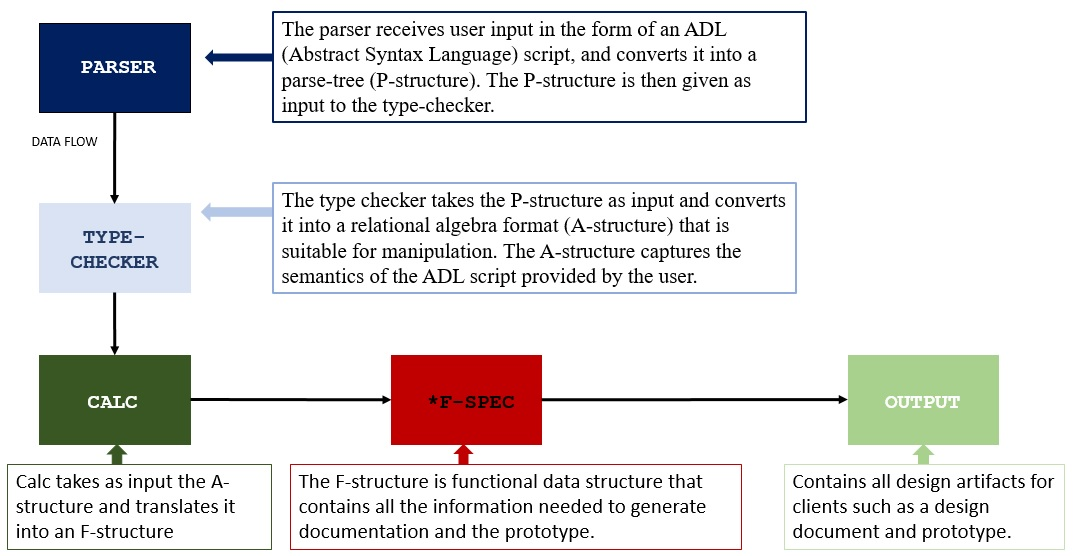
\includegraphics[width=\textwidth]{../figures/ampersand_parts}
    \caption{Components of Ampersand System}~\label{fig:AmpersandParts}
\end{figure}

The context of the work involves investigating how the exec-engine connects to 
the other major components. Additional work goes into determining what degree 
of the old program must be replaced by EFA.
%\section{Business Data Model and Data Dictionary}
%This section is used to 

\begin{figure}[!htb]
\begin{center}
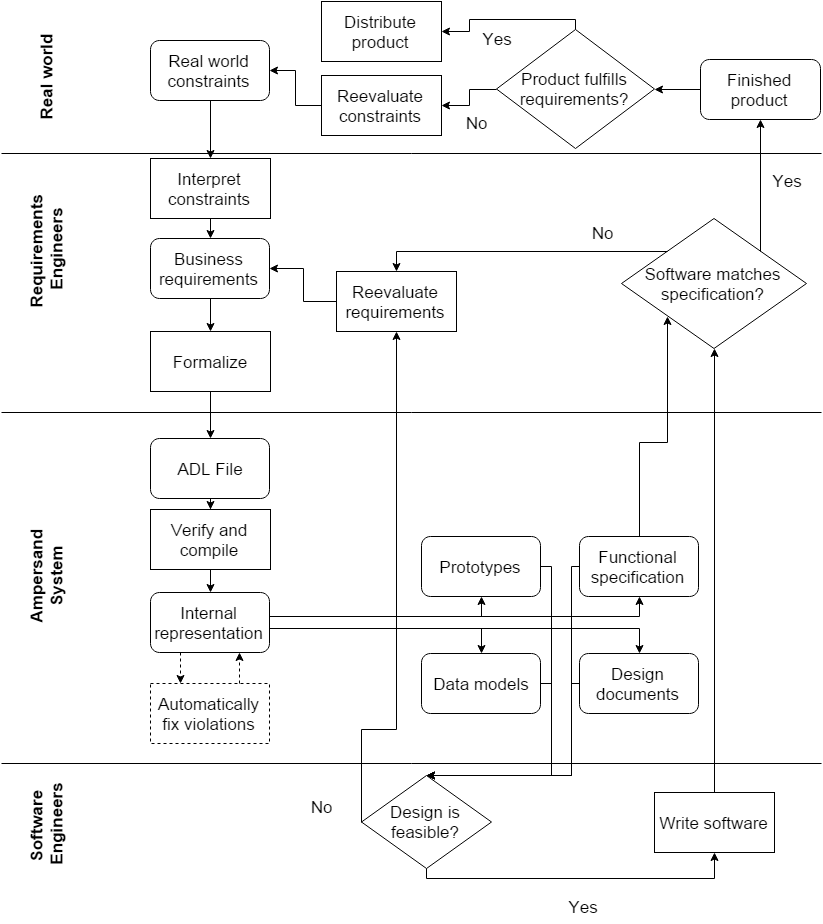
\includegraphics[width=\textwidth]{../figures/business_process}
\caption{Business process diagram representing the role of Ampersand in the
  software design cycle}~\label{fig:BusinessProcess}
\end{center}
\end{figure}

\edcomm{JG}{YT, this diagram needs to be adjusted for the placement of 
prototypes, see Kahl's email}

\edcomm{YT}{The template has a bunch of stuff for this section. But I think this
  diagram is a good summary. Let me know what you guys think. }%

Figure \ref{fig:BusinessProcess} is a simplified view of the software design
cycle, intended to highlight the role of Ampersand in this cycle. This view
omits many of the uses of the design artifacts generated by Ampersand; instead
it focuses mainly on the primary purpose, which is to help create a finished
software system. 

The contribution of this project is denoted with dashed lines. Note that it is
isolated to a process completely internal to Ampersand. It should not affect the
interface to Ampersand.


\begin{longtable}{ |m{4.5cm}|m{1.5cm}|m{7cm}|  }
\hline 
\textbf{Entity} & \textbf{Type} & \textbf{Description} \\
\hline \hline
Real World & Actor & Everything outside of the software system \\ \hline
Requirements engineers & Actor & Stakeholder: end-users\\ \hline 
Ampersand system & Actor & The Ampersand software tool (\ref{sec:Naming}) and
  all of its associated resources. \\ \hline 
Software engineers & Actor & Stakeholder: end-users\\ \hline
ADL File        & Object        & The input to Ampersand, see section 
\ref{sec:Naming} \\ \hline  
Real world constraints  & Object & Driving force for software system \\
Finished product  & Object & The finished software system, including supporting 
documentation and training/services  \\ \hline
Business requirements & Object & Important constraints separated
into logical units, see section \ref{sec:Naming} \\ \hline
Internal representation & Object & The internal representation on which all
  computations are done; this is never exposed to the outside world directly \\ 
  \hline
Prototypes & Object & Resource generated by Ampersand \\ \hline
Data models & Object & Resource generated by Ampersand \\ \hline
Design documents & Object & Resource generated by Ampersand \\ \hline
Functional specification & Object & Resource generated by Ampersand \\ 
\hline
Distribute product & Process & Physical deployment of software and services \\ 
\hline
Re-evaluate
constraints & Process & Constraints deemed not valid and must be 
re-evaluated \\ \hline
Interpret constraints & Process & Turn constraints into business requirements 
\\ \hline
Formalize & Process & Rewrite something in formal language, usually from 
natural language \\ \hline
Re-evaluate
requirements & Process & Requirements deemed not valid and must be re-evaluated
\\ \hline
Verify and compile & Process & Verification consists of type-checking (see 
\ref{sec:Naming}) \\ \hline
Automatically fix violations & Process & Insert the necessary code so that
  generated code will not violated business constraints \\ \hline
Write software & Process & \\ \hline
Error detection & Process & Is this product able to detect inconsistent data 
errors with new contributions? Is the error detection robust enough to catch 
process associated bugs such as cycling, and deadlocks?\\ \hline
Product  fulfills requirements? & Decision & Is the product deemed sufficient 
or accepted? \\ \hline
Software matches specification? & Decision & Does the software meet all of the
  requirements set forth by the formal specification? \\ \hline
Design is feasible? & Decision & Does the software engineer think that the
  design can be implemented in the desired timeframe? \\ 
\hline
 \caption{Description of entities present in figure \\ 
 \ref{fig:BusinessProcess}}
\end{longtable}

\edcomm{JG}{YT, this needs to be adjust via Joosten's comments, as this is 
yours, as per your request -- I wont touch it.}

\section{The Scope of the Product}\label{sec:ScopeOfProduct}
\edcomm{JG}{Scope = work that needs to be done to deliver a product}
EFA require formal proofs and documentation that are provable in addition to 
its implementation; the implementation requires the final product to be able to 
implement an algorithm in Haskell that restores rules made by the user (i.e., 
invariants) and correct any data which have violated these rules. 

The primary deliverable


\section{Functional Requirements}\label{sec:Functional}

\subsection{System Requirements}
%%-----------------------------SIDE EFFECTS---------------------------------%%
{\setlength{\tabcolsep}{6pt} %% Default is 6
    \begin{tabularx}{\textwidth}{>{\bfseries}m{3cm}X}
        Requirement & S1 \\ 
        \midrule
        \endhead
        Description  & Create pure functions with no unintended side effects
        \\	Rationale & The use of a functional programing languages requires 
        that this program be a pure function and does not have side effects, 
        however certain portions of the code requires the execution of side 
        effects to match the behaviour presented by external programs. In these 
        specific instances, the side effects are an intended behaviour.
        \\	Originator & Stakeholder/Developer
        
        \\	Fit Criterion & This behaviour is necessary to produce the results 
        the stakeholders desire
        \\ Test Case & Desired results can be confirmed as they will be 
        reflected in changes that take place in the Ampersand database.
        \\	Customer Satisfaction & 5 - Highest 
        \\	Priority & 5 - Highest 
        \\	Supporting Materials & (Rule Based Design \cite {RBD})
        \vspace{12pt}
    \end{tabularx}
}

%%------------------ MODULES MUST FIT AMPERSAND FRAMEWORK-----------------%%
{\setlength{\tabcolsep}{6pt} %% Default is 6
    \begin{tabularx}{\textwidth}{>{\bfseries}m{3cm}X}
        Requirement & S2 \\ 
        \midrule
        \endhead
        Description  & Added modules must fit within Ampersand's current 
        framework
        \\	Rationale & As Ampersand is a huge system that has weekly additions 
        to prevent conflict and breaking of existing packages/modules, an 
        effort should be made to minimize external dependencies. As EFA will be 
        an internal component of Ampersand, if a package that EFA depends on to 
        function properly is no longer maintained and breaks, it will in turn 
        break Ampersand.
        \\	Originator & Ampersand Creators (i.e. our client)        
        \\	Fit Criterion & Functionality of EFA as an Ampersand internal 
        component.
        \\ Test case & Added modules are tested with cabal build inside of the
        Ampersand system as an internal component (i.e. System testing)
        \\	Customer Satisfaction & 4 - High 
        \\	Priority & 4 - High
        \\	Supporting Materials & Hackage, Dr. Kahl
        \vspace{12pt}
    \end{tabularx}
}
%%----------------------- MACHINE--------------------------------------------%%
{\setlength{\tabcolsep}{6pt} %% Default is 6
    \begin{tabularx}{\textwidth}{>{\bfseries}m{3cm}X}
        Requirement & S3 \\ 
        \midrule
        \endhead
        Description  & Machine-checked proofs
        \\	Rationale & EVA data-types are indexed on Haskell types, and 
        indices are selected in a way that impossible values are eliminated by 
        Haskell's strong type system.
        \\	Originator & Stakeholder/Developer
        
        \\	Fit Criterion & Program compiles and provides an inductive proof 
        that the SQL generated by ECA2SQL is correct
        \\ Test Case & Verified by examination
        \\	Customer Satisfaction & 5 - Highest 
        \\	Priority & 5 - Highest 
        \\	Supporting Materials & Requirement solicitation.
        \vspace{12pt}
    \end{tabularx}
}

\subsection{Project Requirements}
%%-------------------------TYPE CORRECTNESS ----------------------------------%%
{\setlength{\tabcolsep}{6pt} %% Default is 6
    \begin{tabularx}{\textwidth}{>{\bfseries}C{3cm}X}
        Requirement & P1 \\ 
        \midrule
        \endhead
        Description  & Provable Correctness: Haskell like other functional 
        programming languages have 
        a strong type system which can be used for machine-checked proofs.
        \\	Rationale & Curry-Howard correspondence which states that the 
        return type of the function is analogous to a logical theorem, that is 
        subject to the hypothesis corresponding to the types of the argument 
        values that are passed to the function and thus the program uysed to 
        compute that function is analogous to a proof of that theorem.
        \\	Fit Criterion & Provable correctness of the program that is 
        generated.
        \\ Test Cases & Internal structure of ECA rules can be compared to SQL 
        queries through a series of datatype tests, each of which will result 
        in a traceable result or error message
        \\	Priority & 4 - High
        \\	Supporting Materials & Programming language theory, Dr. Kahl
        \vspace{12pt}
    \end{tabularx}
}
%%--------------------------CORRECTNESS OF ECA TO SQL RULES ------------------%%
{\setlength{\tabcolsep}{6pt} %% Default is 6
    \begin{tabularx}{\textwidth}{>{\bfseries}C{3cm}X}
        Requirement & P2 \\ 
        \midrule
        \endhead
        Description  & Generated SQL queries must preserve the semantics of ECA 
        rules.  
        \\	Rationale & The translation would otherwise not be correct, as the 
        rules would be meaningless if their semantics are lost.
        \\	Originator & Ampersand Developers
        \\	Fit Criterion & Generated queries must be provably correct as per 
        client's request.
        \\ Test Cases & Internal structure of ECA rules can be compared to SQL 
        queries through a series of datatype tests, each of which will result 
        in a traceable result or error message
        \\	Priority & 4 - High
        \\	Supporting Materials & Requirements solicitation, Dr. Kahl
        \vspace{12pt}
    \end{tabularx}
}
%%-------------------------ERROR HANDLING---------------------------%%
{\setlength{\tabcolsep}{6pt} %% Default is 6
    \begin{tabularx}{\textwidth}{>{\bfseries}C{3cm}X}
        Requirement & P3 \\ 
        \midrule
        \endhead
        Description  & Be able to process and handle errors on new additions.
        \\	Rationale & For possible future changes to EFA, errors must be 
        processed and handled correctly. Otherwise it could introduce a variety 
        of problems to the Ampersand system and make it difficult to retain EFA 
        as a maintainable component.
        \\	Originator & Ampersand Developers
        \\	Fit Criterion & Errors must be handled correctly
        \\ Test Cases & Manual Testing of individual functions
        \\	Priority & 4 - High
        \\	Supporting Materials & Hackage \cite{hackage}, Dr. Kahl
        \vspace{12pt}
    \end{tabularx}
}

\chapter{Non-functional Requirements}\label{ch:NonFunc}
\begin{figure}[!htb]
	\centering
	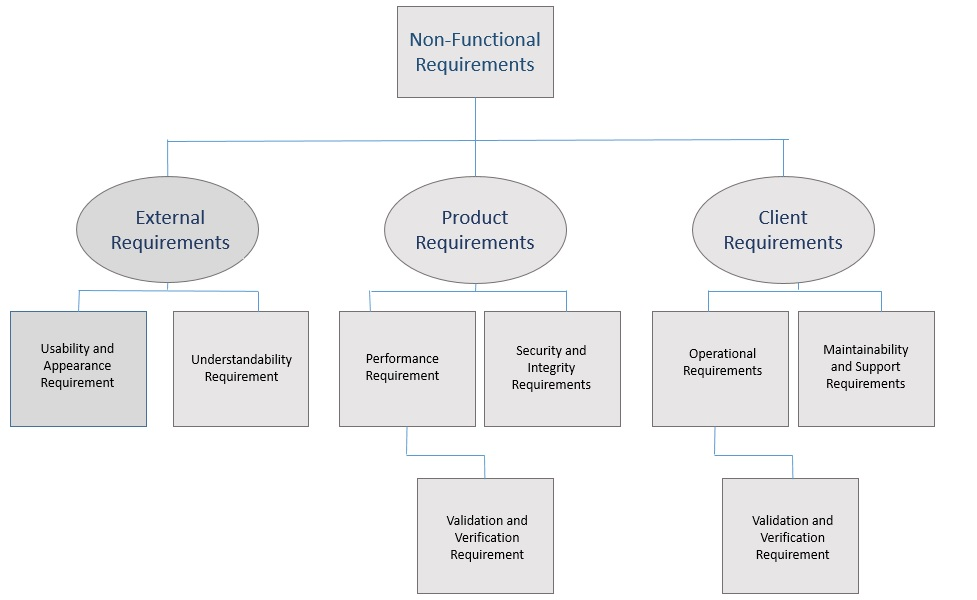
\includegraphics[width=0.8\textwidth]{../figures/NONFUNCTIONAL}
	\caption{Tree of non-functional requirements as it relates to EFA}~\label{fig:figure2}
\end{figure}

\section{Look and Feel Requirements}\label{sec:LookAndFeel}
\begin{itemize}
    \item The product shall comply with Ampersand standards
    \item The product shall appear readable for Ampersand contributors
\end{itemize}

\section{Usability and Humanity Requirements}\label{sec:Usability}

\begin{itemize}
    \item \textit{Efficiency of use} 
        \begin{itemize}
           \item EFA is easy to use for any Ampersand user.
           \item The user can use EFA with accuracy, as they are provided with 
           the option to use EFA's automated service through the users 
           interface.
        \end{itemize}
    \item \textit{Ease of remembering}  
        \begin{itemize}
            \item EFA does not require the user to memorize protocols
        \end{itemize}
    \item \textit{Error rates} 
        \begin{itemize}
            \item EFA eliminates ECA rule violations caused by the user, 
            EFA's implementation is provably correct through Haskell 
            type-checking system.
        \end{itemize}
       
    \item \textit{Feedback} 
        \begin{itemize}
            \item User receive feed-back concerning the ECA rule 
            violations that have been resolved.
        \end{itemize}
    \item \textit{Overall satisfaction in using the product} 
    \begin{itemize}
        \item Users can be confident in using EFA as it is well tested and 
        provides accurate results which the user can confirm.
    \end{itemize}
\end{itemize}

\subsection{Personalization and Internationalization 
Requirements}\label{subsec:Personalization}
EFA is available only in English but can be adapted for other languages in 
later development versions.

\subsection{Learning Requirements}\label{subsec:LearningReq}
EFA has a shallow learning curve, more time is spent learning the Ampersand 
system. No training is necessary to use EFA as long as the user can operate 
Ampersand.

\section{Understandability and Politeness 
Requirements}\label{sec:Understandability}
Conceptually EFA is easy to understand and users will intuitively know what 
this product does for them. To further understandability, EFA feed back uses 
natural language that is familiar to the user and easy to understand. In 
addition, EFA hides all details of its construction from the user and provides 
the user. 

\ds{What are your understandability requirements for this project?}
\edcomm{JG}{kind of addressed}
\subsection{Accessibility Requirements}\label{Accessibility}
EFA is unable to individually confirm to disability requirements as it is an 
internal component of Ampersand.

\section{Performance Requirements}\label{sec:Performance}
\subsection{Speed and latency Requirements}\label{subsec:SpeedReq}
The use of EFA should not result in a noticeable time delay. EFA shall 
not take more than 3 seconds to complete in the worst case scenario.

\subsection{Safety-Critical Requirements}\label{subec:SafetyReq}
EFA will not expose sensitive information in the Ampersand system to outside 
sources or create new vulnerabilities.

\subsection{Precision or Accuracy Requirements}\label{subsec:AccuracyReq}
SQL queries generated by EFA is correct 100\% of the time with full coverage of 
all ECA rules that apply.
\edcomm{JG}{There's more to be added here, cant think of any right now}
 
\subsection{Reliability and Availability Requirements}\label{subsec:AvailReq}
EFA is available for use anytime Ampersand is used. In the event that Ampersand 
fails, then EFA will also be unavailable as it depends on Ampersand generated 
data taken from the user.

\subsection{Robustness or Fault-Tolerance Requirements}\label{subsec:FaultReq}
\edcomm{JG}{Function under abnormal circumstances, what would be considered 
abnormally normal for EFA? No rule violations? It cant function "locally" it 
needs the Ampersand system}

In the absence of ECA rule violations, EFA will continue to function and be on 
stand-by until a rule violation is triggered.
\subsection{Capacity Requirements}\label{subsec:CapacityReq}
Ampersand runs on individual machines; EFA as an internal component of 
Ampersand will be able to deal with any amount of data that Ampersand can 
handle. 
\edcomm{JG}{Dont know the capacity for Ampersand -- it seems to take whatever 
you throw at it }
\subsection{Scalability and Extensibility 
Requirements}\label{subsec:ScalabilityReq}
EFA is capable of handling large volumes of data, and the translation of ECA 
rules to SQL queries requires a standard amount of time. The number of ECA 
rules is expected to expand as Ampersand etches closer to completion. 

\subsection{Longevity Requirements}\label{subsec:LongevityReq}


%%Figure removed - unreferenced and unexplained Figure.

%%	YS
%% 	Does this image aboe (^^) belong here? I believe this is the Figure 5.4 that is related to role of Ampersand in the INDiGO proj
%%	 I suggest the following changes, in support of Dr. Joosten's comments
\edcomm{YS}{ECA rules can have interdependencies, these might be buried deep into the rules. Following a certain course of action under EFA, can trigger a deadlock situation where in the system is not able to come up with the best way to deal with inconsistencies in data. In the above example lets say the system is required to give a 2$ discount to the customer if the total cost(including) of his basket is greater than or equal to $10 and provide free shipping, but if the total cost (after discount ) is less than 10$ then 2$ needs to be added for shipping. This creates an infinite loop where the initial cost of the chair is a discount to $8 but then shipping is applied, and it becomes $10, which is again subjected to the discount. EFA needs to take care of such performance issue that would lead the system into a state if deadlock. EFA must have a run time capability to interrupt and send a message to the user about the existence of such conflicting requirements.
}
\edcomm{JG}{feel free to add that}
%%	I'm not too sure if the example is valid in our case, Does Ampersand automatically detect such conflicting requirements at an
%%	early stage? I've belive the existence of relational algebra can detect such conflicts, but what if they are introduced at run
%%	later, while the information system is in production?

%% Can you guys come up with a better example? The ones we've listed before don't really capture the performance of EFA

\section{Operational and Environmental Requirements}\label{sec:Operational}
\paragraph*{}
Any system that is currently running Ampersand will be able to run this product 
under a new verion and thus no new requirements have been introduced.
\ds{Either explicitly state the current requirements for running Ampersand, or
mention that any system currently running Ampersand will be able to run
the new version and thus no new requirements have been introduced}.

\section{Maintainability and Support Requirements}\label{sec:Support}
\paragraph*{}
All code submitted for this project must be maintainable, which mean it is well 
documented and comes with mathematical proof. This is an essential requirement 
for the future maintenance of Ampersand. EFA must make sure that each 
specification/error is traceable (\cite[2]{derFun}).

\edcomm{who}{Part of the reason that non-functional requirements as essential 
to EFA concerns the requirements for interfacing with Adjacent Systems. Thus 
features concerning how implementation is done which is normally based on the 
choice of the designers is a functional requirement when it comes to EFA }
%%YS - 	I don't think the above commented lines are related to EFA or it maintainability.
%%		I don't think they belong here.
  
\ds{Pull out the explicit requirements and remove the fluff.}

\section{Security and Integrity Requirements}\label{sec:Security}
\edcomm{JG}{this section includes access requirements: who is authorized to access the product. 
Since its open source, anyone can access or change it, it just wont be part of the official source 
code? We're not dealing with sensitive information (there's no confidentiality breach possible..) I 
mean we could name system function name, and user roles but thats a rather short two sentences
	
	There also specificiation of  requried integrity of databases; this is partially applicable, it 
	applies to Ampersand and how it requires a local database but EFA doesn't.. however, it is 
	part of Ampersand. 
	
	We dont have privacy issues.. do we? 
	Audit requirements --- specification of what the product has to do (work?)
	---- we might need audit requirements I mean we could say that if we fed it standard rules it 
	should be able to recognize, translate and fix easily. like if A (subset) B and B (subset C) 
	then A (subset) C. If a is need for b to function, and b is needed by c to function, then by 
	<insert property name> a is required for c.
	
	Immunity requirements: we dont.. really have security, so immunity is confusing.
	
	
}
\paragraph*{}
As an open source project any individual who clones the Ampersand Github has access to source code 
and can manipulate it as they wish. Irrelevant of what changes the user makes locally, it does not 
effect the Github respository, as only developers of Ampersand \big(i.e., our client \big) has 
permission to change source code in the respository. Access to the database and software which 
supports the various functions of Ampersand are run locally and subjected to the security system 
the user has in place on his or her work station.

\ds{The git repository is not the issue here, are there any security/integrity
	concerns for the data you will be handling or for the way your contribution
	will handle data?}
	
\section{Validation and Verification Requirements}\label{sec:Verification}

\edcomm{JG}{ We can distinguish validation from verfication here, like Joosten did, and link how 
validation is required for verification and validation must be done by the user.
		As Joosten specifies that validation is only something that the user can do.. however, does 
		EFA in theory validate the state of the system by fixing inconsistent data? 
		
		Someone help a brother out?What's below cant be all there is}
\paragraph*{}
Validation and verification are important parts of non-functional requirements used to test the 
quality of the final product. Validation is a human activity and requires user input; the rules for 
the software system to follow are provided by the user, and only the user can judge if the rules 
are correct for the system that they are attempting to create. The validation that EFA offers is 
a logical test to confirm that all data sets do not violate the rules that the system follow for 
the model to properly mimic realistic conditions. 

Verification test the accuracy of EFA, and how well it can replicate what the use has in mind 
according to an ECA rule system. Verification is an automated process that confirms correctness 
of the project in accordance to previously validated rules. Furthermore, verification confirms the 
success of ECA rule adoption, and is able to quantify the level of success or failure 
encountered by EFA (\cite{RBD}). 
%TODO{JG}: cite Rule Design (section on verification and validation); then confirm that we can meet 
%these principles or else we need to redefine what these terms are in our project

\ds{What are your explicit verification/validation requirements?}

\section{Legal Requirements}\label{sec:Legal}
The implementation must eventually be included in Ampersand, which is licensed
under GPL3. To comply with this license, all of the implementation code must be
either written by us so we may license it under GPL, or must already be licensed
under GPL, or a compatible license, by its original author. We do not plan to
use existing code, other than as a reference.
\edcomm{YS}{Rephrase this one, I wanted to put forward the idea}%
\edcomm{YT}{I rephrased it more concretely: we have to follow the license agreement of
Ampersand, which appears to be GPL3. That means all the code we include must
either be our own so we can place it under that license, or must already be
under GPL. I don't see any reason we couldn't take code from somewhere if it was
GPL. }%

%%%%%%%%%%%%%%%%%%%%%%%%%%%%%%%%%%%%%%%%%%%%%%%%%%%%%
\chapter{Project Issues}\label{ch:issues}
\section{Open Issues}\label{sec:issues}
Our contribution consists entirely of adding a new feature to Ampersand. There
have been no significant previous efforts to implement this feature within
Ampersand. There are no open issues outside of implementing this feature. 
\edcomm{YS}{Since we're not concerned with any problem or issues associated with Ampersand.}%
\section{Off-the-Shelf Solutions}\label{sec:solutions}
No off the shelf solutions exist for this project.
\section{New Problems}\label{sec:NewProblems}
Our contribution will be entirely internal to Ampersand; it will not affect end
users in terms of the interface to Ampersand or any of the resources that
Ampersand generates. 

The current Ampersand environment will not be affected by our contribution,
since EFA is an additional feature whose functionality will exist on top of
existing functionality; that is, EFA will not affect old functionalities of
Ampersand.

Our contribution will be smoothly intergrated into Ampersand using git and GitHub. 
This transition is not expected to create any problems. 
\edcomm{YS}{Since we're not concerned with any problem or issues associated with Ampersand.}%
\section{Tasks}\label{sec:Tasks}
\begin{itemize}
\item Analyze and the existing software code base and do an impact analysis of our project on the existing software.
\item Propose a solution to the supervisor and product owner.
\item Implement the solution and provide the  annotated source code to the supervisor and the product owner for a review.
\item Incorporate any changes suggested by them and create a pull request in the main Ampersand repository upon successful completion of the task.
\end{itemize}
\edcomm{YS}{Add in any significant task you feel is worth mentioning}%
\section{Migration to the New Product}\label{sec:Migration}
\paragraph*{}
Upon final review by the client and intensive testing, if the client is
satisfied by the quality of code and its maintainability, the implementation
will be made part of the production stream.  This process is quite simple due to
the nature of the project; the core development team of Ampersand is quite
small, and the project is hosted on GitHub; so our migration will consist of
submitting a pull request to the Ampersand repository.
\section{Risks}\label{sec:Risks}
\begin{itemize}
\item The new code must not introduce any 
errors or performance regressions
into Ampersand.
\item The code must satisfy existing tests and 
additional tests written for the new algorithm being implemented.
\end{itemize}

\section{Costs}\label{sec:Costs}
\paragraph*{}
Currently the Ampersand software system is open source and maintained by Tarski
Systems.  All the software subsystems used in Ampersand are also open
source. There will no change in cost as a result of our implementation. The
client (Tarski Systems) will be responsible for managing the cost of
maintenance of the software in the future. All software used in the development
of EFA (GHC, LaTeX, etc.) are open source as well; there is no cost
requirement for any component used.
\ds{You can also mention time costs.}
\section{User Documentation and Training}\label{sec:UserDoc}
\paragraph*{}
 User documentation will accompany EFA which will give a brief explaination concerning 
how EFA works and how users can use EFA to maximize their efficiency. EFA requires minimal 
input from user, but each possible input will be explained thoroughly and various examples will be 
provided in a step by step tutorial to help familiarze the user with EFA. Furthermore, a 
practice simulation will be in place for the user. The test will include a well documented default 
script which the user can compile to try out different priority options. The manual will include 
pictures as a type of visual guide concerning what the screen should look like from beginning to 
end. The documentation will likely be part of the Ampersand documentation, but for the purposes of 
this project, it will be submitted independently. 

\section{Waiting Room}\label{sec:Waiting}
Our project consists of implementing a single feature. There are no other
features that even touch the scope of this project. Therefore, there are no
requirements which will not be satisfied as a part of the initial release.

%% \section{Ideas for Solutions}\label{sec:Solutions}
\edcomm{YT}{Not really relevant... our 'solution' consists of implementing a
  known algorithm. Maybe we could put something here if we had started
  implementing and could even thing about this...}

\ds{Overall comment: Too verbose. Throughout the document
you use a lot of words to say very little.}

\bibliographystyle{alpha}
\bibliography{SRS}
\end{document}










